\section{Struttura dati}
Per quanto riguarda il flusso di un ordine all’interno del sistema si considera che immediatamente dopo l’ordinazione da parte del cliente viene assegnata una priorità per tale ordine, gli ordini vengono così raccolti nella struttura dati principale con l’etichetta della priorità. Successivamente, se la cucina lo richiede, l'ordine con la priorità più elevata viene spostato nella coda di preparazione della rispettiva postazione di lavoro.


\begin{figure}[htbp]
	\centering
	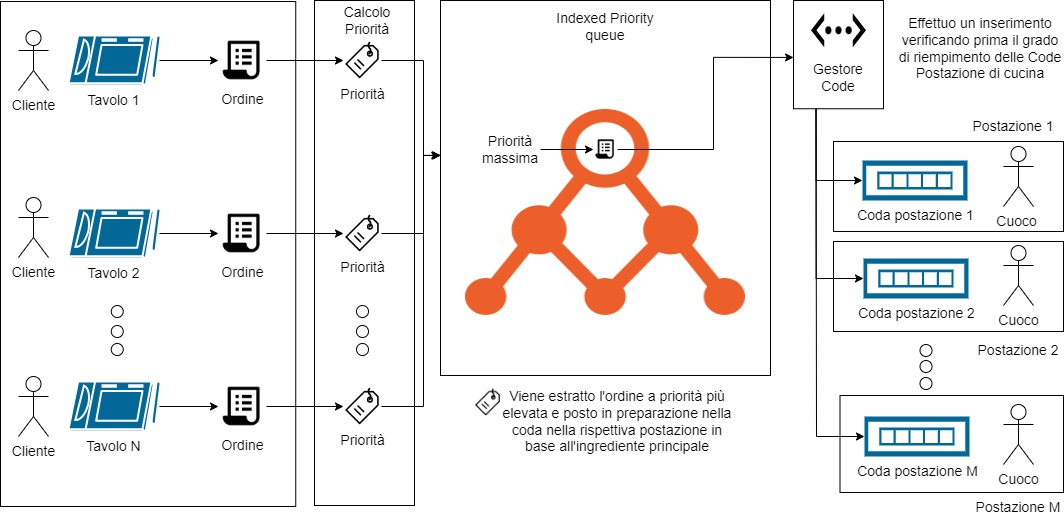
\includegraphics[scale=0.4]{iterazione2/images/Algoritmo_struttura.jpg}
	\caption{Strutture dati dell'algoritmo\label{fig:algoritmo_struttura}}
\end{figure}

Si rendono quindi necessarie due tipi di strutture dati:
\begin{itemize}
	\item Struttura dati principale: Indexed priority queue;
	\item Struttura dati delle postazioni: Coda (queue).
\end{itemize}

\subsection{Indexed priority queue}
Struttura dati che estende il concetto di coda con priorità aggiungendo la possibilità di accedere in tempo costante agli elementi presenti in coda per compiere operazioni quali la modifica dei parametri, l’aggiornamento della priorità o la rimozione dell’ordine (che altrimenti presenterebbe costo lineare).
Viene implementata per mezzo di una combinazione di una coda con priorità (max heap) e un dizionario (hashtable) che tiene traccia della posizione di ogni elemento all'interno della coda.

\paragraph{Analisi complessità:}
La complessità temporale è correlata a quella di un heap binario, potenziato dall’accesso diretto agli elementi tramite dizionario, di conseguenza:
\begin{itemize}
	\item creazione: O(n);
	\item inserimento e rimozione: O(log n);
	\item modifica priorità: O(log n);
	\item accedere a un elemento: O(1).
\end{itemize}

\paragraph{Requisiti funzionali:}
\begin{itemize}
	\item Gestione degli ordini con priorità: funzionalità chiave della struttura dati, gli ordini ricevono una priorità prima di entrare nella coda a priorità indicizzata;
	\item Fornire l'ordine con priorità più elevata: la struttura dati deve essere in grado di fornire alla cucina l'ordine con la priorità più alta quando richiesto;
	\item Accesso, modifica e rimozione degli ordini: la coda a priorità deve poter fornire la possibilità di implementare la funzionalità che consente ai clienti di accedere, modificare o rimuovere il proprio ordine (nelle prossime iterazioni);
	\item Flessibilità nella modifica delle priorità: la struttura deve garantire una certa flessibilità alla modifica delle priorità degli ordini, poiché le priorità possono cambiare per conto dei clienti, della cucina e a intervalli regolari di tempo.
\end{itemize}

\paragraph{Requisiti non funzionali:}
\begin{itemize}
	\item Tempo di risposta rapido: l’ordine con priorità più elevata deve essere fornito in tempo rapido alla cucina senza ritardi;
	\item Tempo di accesso, modifica e rimozione ragionevole: il cliente deve poter effettuare operazioni senza complicazioni in tempi ragionevoli, mantenendo un’esperienza di utilizzo piacevole;
	\item Scalabilità: La struttura dati deve essere in grado di gestire un grande volume di ordini, adattandosi alle variazioni nella domanda senza compromettere le prestazioni;
	\item Flessibilità alle modifiche: requisito non funzionale relativo alla flessibilità e alla manutenibilità del sistema.
\end{itemize}

\subsection{Coda (queue)}
Struttura dati lineare che segue il principio "First In, First Out" (FIFO), ossia il principio per il quale il primo elemento che entra nella coda è poi il primo che esce.
\paragraph{Analisi complessità:}
\begin{itemize}
	\item inserimento in coda: O(1);
	\item rimozione della testa: O(1);
	\item verifica stato: O(1) se vuota, O(n) altrimenti.
\end{itemize}

\paragraph{Requisiti funzionali:}
\begin{itemize}
	\item Funzionamento FIFO: La coda deve garantire il corretto funzionamento FIFO (First In, First Out), indipendentemente dalle priorità degli ordini;
	\item Soglia di attivazione: Il sistema deve permettere di configurare una soglia di valore minimo di attivazione per la coda, al di sotto della quale la postazione non viene attivata;
	\item Soglia critica di intasamento: Il sistema deve permettere di configurare una soglia di valore critico, oltre la quale la postazione diventa intasata e richiede operazioni per ridurre il carico.
\end{itemize}

\paragraph{Requisiti non funzionali:}
\begin{itemize}
	\item Lunghezza finita della coda: Il sistema deve gestire una coda con una lunghezza finita, limitata dalla capacità della postazione di lavoro;
	\item Tempo massimo di attesa in coda: Il sistema deve garantire che gli ordini non rimangano in coda di preparazione per troppo tempo prima di essere elaborati;
	\item Attivazione anticipata della postazione: In casi di eccessivo ritardo nella preparazione degli ordini, il sistema può attivare una postazione di lavoro anche se è al di sotto della soglia minima di attivazione.
\end{itemize}

\clearpage
